\documentclass[12pt,a4paper]{report}
\usepackage[portuges,brazil]{babel}
\usepackage[latin1]{inputenc}
\usepackage[T1]{fontenc}
\usepackage{graphicx}
\usepackage{indentfirst}
\usepackage{fancyheadings}


% fonts
\usepackage{palatino}
%\usepackage{courier}


% math
\usepackage{amsmath, amsthm, amssymb}
\usepackage{latexsym}
%\usepackage{enumerate}
%\usepackage{float}
%\usepackage{floatflt}
%\usepackage{array}
%\usepackage{longtable}
\newtheorem{teor}{Teorema}%[section]
\newtheorem{coro}[teor]{Corolário}
\newtheorem{prop}[teor]{Proposição}
\newtheorem{lema}[teor]{Lema}
\newtheorem{conj}[teor]{Conjectura}
\newtheorem{fato}[teor]{Fato}
\newtheorem{defi}[teor]{Definição}
\newtheorem{exem}[teor]{Exemplo}


% probability
\usepackage{xspace} 
\newcommand{\Pro}{\xspace\protect{\ensuremath{\textup{Pr}}}\xspace}
\newcommand{\Esp}{\xspace\protect{\ensuremath{\textup{E}}}\xspace}


% algorithms
\usepackage[ruled]{algorithm}
\usepackage[noend]{algorithmic}
% Cormen algorithms
\usepackage{clrscode}

% hiperlinks
\usepackage[backref,pdfpagemode=UseOutlines,colorlinks=true,
a4paper,breaklinks=true,hyperindex,linkcolor=red,
anchorcolor=black,citecolor=green,filecolor=magenta,
menucolor=red,pagecolor=red,urlcolor=blue,bookmarks=true,
bookmarksopen=true,pdfpagelayout=SinglePage,
pdfpagetransition=Dissolve]{hyperref}


% format
\setlength{\parskip}{.2cm}
\setlength{\textwidth}{16cm}
\setlength{\textheight}{23 cm}
\setlength{\topmargin}{0cm} 
\setlength{\oddsidemargin}{0.5cm}
\setlength{\evensidemargin}{0.5cm} 


\begin{document}

\vspace*{\stretch{1}}

\begin{center}
\noindent \rule{\linewidth}{.1cm}

\vspace*{1cm}

{\LARGE \textsf{Controle no roteamento de rotas utilizando o protocolo BGP}}

\vspace*{1cm}

{\Large \textsf{Gilson Gabriel Zozias de Santana}}

\vspace*{1cm}

\noindent \rule{\linewidth}{.1cm}

\vspace*{1cm}

{\large

\textbf{Projeto de gradua\c{c}\~{a}o apresentado ao} \\
\textbf{Departamento de Computa\c{c}\~{a}o e Estat\'{i}stica da} \\
\textbf{Universidade Federal de Mato Grosso do Sul, para} \\
\textbf{obten\c{c}\~{a}o do grau de Bacharel em Ci\^encia da Computa\c{c}\~ao}

}

\vspace*{1cm}

\begin{figure}[htb]
  \begin{center}
    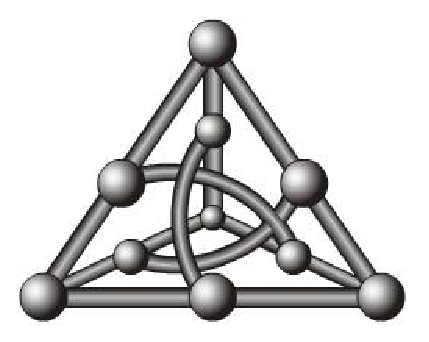
\includegraphics{Imagens/grafo}
  \end{center}
\end{figure}
\vspace{2 cm}

\textbf{Orientador: Prof.~Ronaldo Alves Ferreira}

\vspace*{\stretch{2}}

Campo Grande, Julho de 2018

\end{center}

\newpage

\chapter*{Resumo}
A Internet transformou-se, ao longo dos anos, em um dos meios tecnol\'ogicos mais disseminados mundialmente. Onde os provedores de servi\c{c}os de internet(ISP) come\c{c}aram a modificar as configura\c{c}\~oes de roteamento para apoiar pol\'iticas de roteamento, no qual o propriet\'ario do roteador que controlava quais as rotas foram escolhidas e quais rotas foram propagadas para os vizinhos. Portanto esta proposta usa um protocolo de arquitetura de rede usando o Border Gateway Protocol(BGP) que atende aos requisitos para conectar, monitorar e analisar o tr\'afego entre os clientes desses provedores. Este artigo apresenta um estudo dos aspectos que envolvem o roteamento usando o protocolo BGP, como os seus recursos, e escolhas de decis\~oes econ\^omicas e pol\'iticas envolvidas no roteamento. O resultado deste trabalho foi usado na implanta\c{c}\~ao de um ambiente, onde podemos monitorar o operadores fornecendo os fluxos de dados.

\newpage
\tableofcontents
\newpage

\pagestyle{fancy}
\pagenumbering{arabic}
\renewcommand{\chaptermark}[1]{\markboth{#1}{}}
\renewcommand{\sectionmark}[1]{\markright{\thesection\ #1}}

\lhead[\fancyplain{}{\bfseries\leftmark}]{\fancyplain{}{\bfseries\leftmark}}
\rhead[\fancyplain{}{\bfseries\thepage}]{\fancyplain{}{\bfseries\thepage}}
\cfoot{\fancyplain{\bfseries\thepage}{\scshape facom-ufms}}
\setlength{\footskip}{\dimexpr\headsep+1.5\baselineskip+.4pt}
\setcounter{page}{1}


\chapter{Introdu\c{c}\~ao}
A defini\c{c}\~ao simples de Internet \'e que representa uma cole\c{c}\~ao de redes interconectadas, enquanto os roteadores podem ser definidos, como a intersec\c{c}\~ao que liga essas redes, ou seja, os pontos que possibilitam essa ponte. Estes, por sua vez, est\~ao organizados de forma hier\'arquica, onde alguns roteadores s\~ao utilizados para trocar dados entre grupos de redes controlados pelo mesmo dom\'inio, enquanto outros roteadores fazem tamb\'em a comunica\c{c}\~ao entre dom\'inios. Um grupo de redes IP, sobre uma ger\^encia t\'ecnica e que compartilham uma mesma pol\'itica de roteamento se chama sistema aut\^onomo (AS).

O roteamento \'e a forma mais importante para a entrega de pacotes de dados entre roteadores na internet, atrav\'es de uma infraestrutura de redes interconectadas. Para tanto, o roteamento executa o processamento de rotas para um determinado sistema de comunica\c{c}\~ao, em que s\~ao necess\'arios dois elementos: tabelas de roteamento e protocolos de roteamento. As tabelas de roteamento s\~ao registros de endere\c{c}os de destino associados as m\'etricas para alcan\c{c}ar esse destino, podendo conter outras informa\c{c}\~oes. Os protocolos de roteamento determinam os conte\'udos das tabelas de roteamento, ou seja, eles ditam como a tabela \'e montada e com quais informa\c{c}\~oes ela \'e composta. Existem dois tipos de algoritmos atualmente em uso, pelos protocolos de roteamento: o algoritmo baseado em Vetor de Dist\^ancia (\textit{Distance-Vector Routing Protocols}) e o algoritmo baseado no Estado de Enlace (\textit{Link State Routing Protocols}).

Todos os protocolos de roteamento realizam as mesmas fun\c{c}\~oes b\'asicas. Eles determinam a melhor rota para cada destino e distribuem as informa\c{c}\~oes de roteamento entre os sistemas da rede. A forma pela qual \'e decidida a melhor rota \'e o que determina a diferen\c{c}a entre os protocolos de roteamento existentes, que podem ser internos ou externos. No protocolo de roteamento interno, os roteadores que s\~ao utilizados para trocar informa\c{c}\~oes dentro do sistemas aut\^onomos, s\~ao chamados de roteadores internos (\textit{internal routers}) e podem usar uma variedade de protocolos de roteamento interno (\textit{Interior Gateway Protocols - IGPs}). Dentre eles est\~ao: RIP, IGRP, EIGRP, OSPF, sendo esses \'ultimos os mais usuais. J\'a no protocolo de roteamento externo, os roteadores que trocam dados entre sistemas aut\^onomos s\~ao chamados de roteadores externos (\textit{external routers}), no qual utilizam protocolos tal como o BGP (\textit{Border Gateway Protocol}). Para este tipo de roteamento s\~ao considerados basicamente cole\c{c}\~oes de prefixos CIDR (\textit{Classless Inter Domain Routing}) identificados pelo n\'umero de um sistema aut\^onomo.

Antigamente, o caminho mais curto do roteamento era tipicamente usado. Ao longo do tempo, como a internet tornou-se mais comercializada e privatizada, prestadores de servi\c{c}os de internet (\textit{ISPs}) come\c{c}aram a ter interesses em controlar o tr\'afego de dados por raz\~oes econ\^omicas e pol\'iticas. Com isso o protocolo BGP nasceu da necessidade dos ISPs de controlar a sele\c{c}\~ao e a propaga\c{c}\~ao de rotas. O resultado \'e um protocolo em que a maioria da complexidade est\'a no processo de decis\~ao e as pol\'iticas utilizadas para influenciar nas decis\~oes.

O primeiro objetivo deste projeto \'e estudar detalhadamente o que acontece com o funcionamento do protocolo BGP. Com isto, ser\'a feita uma an\'alise do ambiente de redes visando avaliar os comportamentos poss\'iveis, suas causas e estrat\'egias. Para demonstrar as variedades de t\'ecnicas a fim de fornecer o controle de roteamento do protocolo BGP, foi realizada uma simula\c{c}\~ao baseada em um ambiente real, com quatro backbones: RNP (Rede Nacional de Ensino e Pesquisa), EBT (Embratel), I2 (Internet Comercial 2), BF (Backbone Final). Onde temos relacionamentos entre eles vistos na Figura \ref{fig:Ambiente do projeto}. A implementa\c{c}\~ao do ambiente foi realizado no roteador de software BIRD para o plano de controle e o Kernel Linux para o plano de dados. O Cap\'itulo 2 faz uma an\'alise do protocolo de roteamento interno usado no projeto. No Cap\'itulo 3 traz uma an\'alise do protocolo BGP, tal como o processo de sele\c{c}\~ao de rotas, importa\c{c}\~ao e exporta\c{c}\~ao de rotas, e detalha a import\^ancia das pol\'iticas no protocolo BGP. No Cap\'itulo 4 mostraremos o projeto e a sua implementa\c{c}\~ao. O Cap\'itulo 5 apresenta a avalia\c{c}\~ao da implementa\c{c}\~ao do trabalho. Finalmente, o Cap\'itulo 6 traz a conclus\~ao deste projeto.

\begin{figure}[!htb]
 \centering
 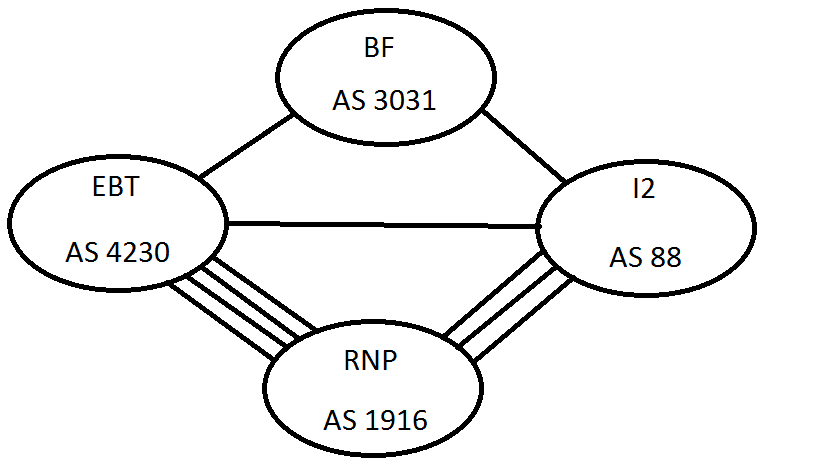
\includegraphics[width=0.5\textwidth]{Imagens/Ambiente}
  \caption{\label{fig:Ambiente do projeto} Ambiente do projeto simulado, com o relacionamento de quatro sistemas aut\^onomos , e seus respectivos n\'umeros}
\end{figure}


\chapter{Roteamento Interno}

Neste cap\'itulo do trabalho s\~ao abordados conhecimentos b\'asicos do protocolo de roteamento interno utilizado no projeto.

Um protocolo de roteamento intra-AS \'e usado para determinar como \'e realizado o encaminhamento de pacotes dentro de um sistema aut\^onomo. Protocolos de roteamento intra-AS tamb\'em s\~ao denominados como protocolos de roteadores internos IGP. Um AS agrupa roteadores que est\~ao sob o mesmo controle administrativo. Ou seja, operados pelo mesmo ISP ou uma mesma corpora\c{c}\~ao. Todos os roteadores do mesmo AS utilizam o mesmo algoritmo de roteamento, no caso deste projeto, o algoritmo utilizado \'e o OSPF (\textit{Open Shortest Path First)}. 

O OSPF \'e um protocolo de roteamento din\^amico. Seu desenvolvimento inicial come\c{c}ou em 1987 pelo Grupo de Trabalho do OSPF da IETF (\textit{Internet Engineering Task Force).} O protocolo \'e aberto, ou seja, de dom\'inio p\'ublico, padronizado pelo IETF, independente e n\~ao propriet\'ario, podendo ser utilizado gratuitamente por qualquer fabricante. 

O OSPF \'e um protocolo de estado de enlace. Poder\'iamos pensar em um link como sendo uma interface no roteador. O estado do enlace \'e uma descri\c{c}\~ao dessa interface e de sua rela\c{c}\~ao com seus roteadores vizinhos. Uma descri\c{c}\~ao da interface incluiria, por exemplo, o endere\c{c}o IP da interface, a m\'ascara, o tipo de rede a que est\'a conectado, os roteadores conectados a essa rede e assim por diante.\cite{Kurose:2012:CNT:2584507} A cole\c{c}\~ao de todos esses v\'inculos formariam um banco de dados.

Toda rota distribu\'ida pelo OSPF possui um endere\c{c}o de destino e uma m\'ascara de rede. O protocolo OSPF encaminha dados baseados no endere\c{c}o IP de destino encontrado no cabe\c{c}alho do pacote IP. O OSPF detecta qualquer altera\c{c}\~ao da topologia e calcula novas rotas sem loop ap\'os um per\'iodo de converg\^encia. Todos os roteadores executam o algoritmo do protocolo OSPF em paralelo. Cada roteador constr\'oi uma \'arvore de menor caminho, com si mesmo como raiz. Esta \'arvore de menor caminho fornece rotas para cada destino no sistema aut\^onomo.\cite{Kurose:2012:CNT:2584507}


\section{Algoritmo do caminho mais curto}

O protocolo OSPF usa o algoritmo do caminho mais curto para criar e calcular o caminho mais r\'apido para todos os destinos conhecidos. O caminho mais curto \'e calculado com o uso do algoritmo Dijkstra. O algoritmo do OSPF por si s\'o possui um n\'ivel muito alto de complexidade, de forma simplificada as v\'arias etapas desse algoritmo s\~ao:

\begin{enumerate}
\item Ap\'os a inicializa\c{c}\~ao ou qualquer altera\c{c}\~ao nas informa\c{c}\~oes de roteamento, um roteador gera um an\'uncio de estado de enlace. Este an\'uncio representa a cole\c{c}\~ao de todos os dados de estados de enlace nesse roteador.
\item Todos os roteadores trocam essas informa\c{c}\~oes. Cada roteador que recebe uma atualiza\c{c}\~ao de estado de enlace deve armazenar uma c\'opia em seu banco de dados de estados de enlace e, em seguida, propagar a atualiza\c{c}\~ao para outros roteadores.
\item Depois que o banco de dados de cada roteador for preenchido, o roteador ir\'a calcular uma \'arvore de caminho mais curto para todos os destinos. O roteador usa o algoritmo de Dijkstra a fim de calcular a \'arvore de caminho mais curto. Os destinos, o custo associado e o pr\'oximo salto para alcan\c{c}ar esses destinos formam a tabela de roteamento IP.
\item No caso de n\~ao ocorrer nenhuma altera\c{c}\~ao na rede OSPF, como o custo de um enlace ou uma rede que est\'a sendo adicionada ou exclu\'ida. Todas as altera\c{c}\~oes que ocorrem s\~ao comunicadas por meio de pacotes de estado de enlace, e o algoritmo de Dijkstra \'e executado novamente com o intuito de localizar os caminho mais curtos.

\end{enumerate}

O algoritmo coloca cada roteador na raiz de uma \'arvore e calcula o caminho mais curto para cada destino com base no custo cumulativo necess\'ario para alcan\c{c}ar esse destino. Cada roteador ter\'a sua pr\'opria exibi\c{c}\~ao da topologia, embora todos os roteadores construam uma \'arvore de caminho mais curta usando o mesmo banco de dados de estado de enlace, no qual cada roteador repete periodicamente o algoritmo acima.\cite{Kurose:2012:CNT:2584507} 

O custo (tamb\'em chamado de m\'etrica) de uma interface no OSPF \'e uma indica\c{c}\~ao da sobrecarga necess\'aria para enviar pacotes atrav\'es de uma determinada interface. O custo de uma interface \'e inversamente proporcional \`a largura de banda dessa interface. Uma largura de banda maior indica um custo mais baixo.

\section{Interfaces OSPF}

Outra id\'eia importante no OSPF \'e que interfaces usadas para trocar informa\c{c}\~oes com vizinhos OSPF t\^em tipos diferentes. Os dois importantes s\~ao:

\begin{enumerate}
\item Uma interface de broadcast OSPF est\'a conectada a uma rede compartilhada, como Ethernet.
\item Uma interface ponto a ponto OSPF est\'a conectada a um link onde s\'o pode haver um \'unico roteador OSPF em cada extremidade.
\end{enumerate}

A raz\~ao para os v\'arios tipos de interface \'e certificar-se de que todos os roteadores saibam sobre todas as rotas de todos os outros roteadores. Em links ponto-a-ponto, n\~ao h\'a nenhum mist\'erio, os dois roteadores sabem que eles s\~ao os \'unicos roteadores OSPF no link e assim eles trocam rotas uns com os outros\cite{rfc2328}.

\section{\'Areas OSPF}

As \'areas no OSPF s\~ao cole\c{c}\~oes de roteadores agrupados. Com exce\c{c}\~ao dos roteadores de borda de \'area, os roteadores OSPF em uma \'area n\~ao s\~ao vizinhos com roteadores em outras \'areas. Entre outras raz\~oes, as \'areas foram usadas para dimensionar grandes redes OSPF. 

Quando o poder de processamento dos roteadores era mais fraco do que s\~ao hoje, uma regra geral era manter uma \'area OSPF para n\~ao mais de 50 roteadores. Isso manteria o n\'umero de c\'alculos de caminho mais curtos OSPF e atualiza\c{c}\~oes de banco de dados para um valor gerenci\'avel \`a medida que as interfaces foram para cima e para baixo, as rotas foram aprendidas e retiradas, e assim por diante. Em redes modernas, n\~ao \'e incomum escalar para mil roteadores ou mais.

Embora a escala n\~ao seja uma boa raz\~ao para implementar v\'arias \'areas, as \'areas OSPF ainda s\~ao \'uteis como limites administrativos em uma rede. Por exemplo: a recapitula\c{c}\~ao e a agrega\c{c}\~ao da rota (substituindo v\'arias rotas pequenas com uma rota maior que as cobre) s\'o podem acontecer nos limites da \'area OSPF. Nem todos os roteadores precisam saber sobre todas as outras rotas dispon\'iveis em uma rede. Usando os conceitos de \'areas OSPF, \'e poss\'ivel injetar uma rota padr\~ao representando todas as rotas fora da \'area local.

A \'area mais importante do OSPF \'e a \'area de backbone, tamb\'em conhecida como \'area 0. A \'area de backbone \'e a \'area que todas as \'areas OSPF devem percorrer para chegar outras \'areas. Por exemplo, como foi desenvolvido no projeto, temos a \'area 0 e a \'area 1 para cada sistema aut\^onomo. Na \'area 0 est\~ao todas as interfaces que est~ao conectados diretamente com dois sistemas auton\^omos. A \'area 1 \'e representada pelas interfaces que est\~ao conectadas com roteadores pertencentes \`a mesma rede\cite{rfc2328}. Embora os roteadores OSPF dentro de uma \'area saibam tudo o que h\'a para saber sobre a topologia de rede, as informa\c{c}\~oes de topologia est\~ao ocultas nas bordas da \'area.

\section{Vantagens do protocolo OSPF}

Ap\'os apresentarmos algumas caracter\'isticas do protocolo OSPF, apresentaremos algumas vantagens deste protocolo, a fim de demonstrar o porque a maioria dos especialistas em rede preferem os protocolos por estado de conex\~ao.

\begin{enumerate}
\item Converg\^encia R\'apida e sem Loop : Enquanto os protocolos vetor-dist\^ancia convergem proporcionalmente ao n\'umero de n\'os na rede. Al\'em disso, nos protocolos vetor-dist\^ancia, a mensagem \'e proporcional ao n\'umero de destinos, se a rede \'e muito grande, cada mensagem vai ter que ser subdividida em v\'arios pacotes, diminuindo mais ainda a velocidade de converg\^encia. Ainda, nos protocolos de estado do link imediatamente ap\'os a transmiss\~ao e c\'alculo, todas as rotas da rede est\~ao sanadas, isto \'e, n\~ao h\'a loops nem contagem ao infinito.
\item Suporte a v\'arias m\'etricas : O OSPF V.2 suporta v\'arios tipos de m\'etrica, de forma que a decis\~ao sobre o menor caminho pode ser tomada em rela\c{c}\~ao ao tempo, ao custo por bit ou confiabilidade. Tornando, portanto, a escolha do melhor caminho mais flex\'ivel, uma vez que cada meio tem caracter\'isticas diferentes. Foi ent\~ao criada uma extens\~ao indicando o tipo de m\'etrica usada num determinado pacote, para que o n\'o que o recebeu n\~ao use uma outra m\'etrica no seu envio e prejudique o roteamento provocando loops ou atrasos. Esta extens\~ao s\'o \'e suportada na vers\~ao 2 do OSPF.
\item Caminhos m\'ultiplos : Nem sempre a melhor rota entre X e Y deve ser a \'unica a ser utilizada, pois isto pode implicar em sua sobrecarga. An\'alises matem\'aticas provaram que a divis\~ao do tr\'afico em duas rotas \'e muito mais eficiente. Isto, apesar de fazer com que as filas em n\'os intermedi\'arios fiquem desiguais, elas s\~ao reduzidas no n\'os. Al\'em disto, se todos escolhessem uma \'unica rota e ela ficasse indispon\'ivel, haveria um grande "re-roteamento" para outro caminho, possivelmente o congestionando. Mas se o tr\'afico fosse separado em v\'arios caminhos, n\~ao haveria muito transtorno caso uma determinada rota ficasse inacess\'ivel. O algoritmo que realiza este tipo de análise \'e bastante complexo, pois, como dificilmente uma fonte e um destino tem duas rotas poss\'iveis exatamente iguais, \'e feita uma an\'alise se as rotas s\~ao suficientemente iguais. Al\'em disto, deve-se decidir a fra\c{c}\~ao do tr\'afico que deve ser enviado em cada uma delas.
\end{enumerate}


\chapter{Protocolo BGP}
O Border Gateway Protocol (Protocolo de Roteamento de Borda - BGP) \'e um protocolo de roteamento entre sistemas aut\^onomos do tipo vetor de dist\^ancia (\textit{Distance-Vector}). Criado em 1989 com o intuito de administrar os di\'alogos entre os roteadores, e de suportar as diferentes infraestruturas j\'a existentes, provendo escalabilidade, flexibilidade e redund\^ancia, al\'em de possibilitar a cria\c{c}\~ao de pol\'iticas de roteamento que respeitassem as particularidades e os anseios de cada uma das organiza\c{c}\~oes que se conectam com a Internet. BGP \'e o protocolo usado para troca de informa\c{c}\~oes sobre roteamento da internet e ele \'e usado por ISP's. V\'arios clientes compartilham o mesmo AS de um ISP, dessa forma, nos roteadores de borda do AS do ISP \'e usado o BGP para trocar informa\c{c}\~oes de rotas com a internet para seus clientes. Para que as informa\c{c}\~oes sejam trocadas a partir do protocolo BGP, \'e feito um acordo, sem levar em considera\c{c}\~ao o custo da comunica\c{c}\~ao, onde esse acordo \'e chamado de peering. O protocolo BGP pode ser usado de duas maneiras: eBGP(External BGP) e iBGP(Internal BGP).

\begin{figure}[!htb]
 \centering
 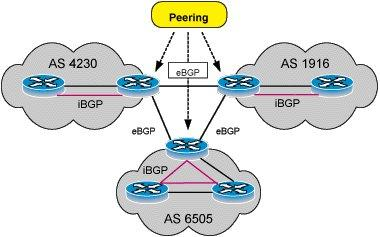
\includegraphics[width=0.5\textwidth]{Imagens/figura2BGP.jpg}
  \caption{\label{fig:figura2BGP}  Uso do iBGP e do eBGP.\cite{Frederico}}
\end{figure}

Geralmente um sistema aut\^onomo possui v\'arios roteadores, em que esses roteadores podem trocar informa\c{c}\~oes. Para que isso aconte\c{c}a, os roteadores devem usar o protocolo BGP interno (iBGP). J\'a quando dois roteadores de sistemas aut\^onomos diferentes(roteadores de borda), utiliza-se o protocolo BGP externo (eBGP). O BGP usa os mesmos tipos de mensagem nas sess\~oes iBGP e eBGP, mas as regras para quando enviar cada mensagem e como interpretar cada mensagem diferem ligeiramente. O protocolo BGP possui um atributo chamado \textit{path}, que \'e o caminho como uma lista de todos os sistemas aut\^onomos que precisam ser percorridos, para alcan\c{c}ar o local onde o prefixo foi anunciado, um meio pelo qual os dispositivos de roteamento BGP evitam loops. Por diferen\c{c}as entre os protocolos iBGP e o eBGP, eles podem ser considerados dois protocolos separados.

\section{BGP Interno}
O objetivo do protocolo iBGP \'e fornecer um meio pelo qual os an\'uncios de rotas eBGP possam ser encaminhados em toda a rede, por\'em deve haver algum protocolo IGP que permite que os dois vizinhos alcancem um ao outro. Como o tr\'afego do iBGP n\~ao modifica o atributo \textit{path} durante os an\'uncios, \'e necess\'ario a preven\c{c}\~ao de loops na rede, e para evitar esses loops de roteamento dentro de um sistema aut\^onomo, \'e essencial que a rede seja de malha completa(todos os roteadores conectado com todos).

\begin{figure}[!htb]
 \centering
 \includegraphics[width=0.5\textwidth]{Imagens/rr-fullmesh}
  \caption{\label{fig:rr-fullmesh} Exemplo de um rede de malha completa iBGP.\cite{EscalandoBGP}}
\end{figure}

Nesta topologia, todos os roteadores usados em iBGP devem ser conectados juntos como malha completa. Esse tipo de configura\c{c}\~ao \'e complexo e dif\'icil de configurar. A complexidade de criar uma topologia full-mesh \'e exponencial e pode ser alcan\c{c}ado atrav\'es da formula\cite{rfc4271} : \[ n*(n-1)/2 \]
Sendo \textit{n} a quantidade de roteadores, e o resultado da express\~ao o n\'umero de peerings necess\'arios para os roteadores se conectarem numa malha completa. Ou seja, em um cen\'ario com 25 roteadores, \'e necessario a cria\c{c}\~ao de 300 peerings. Outro problema pode ser, quando se torna necess\'ario adicionar um roteador na topologia, precisaria atualizar todos os roteadores na topologia iBGP para este roteador. Um caso para reduzir a complexidade dessa topologia, torna-se necess\'ario utilizar o conceito de refletor de rotas (\textit{router reflector}).
\\
\\
\\
\\
\begin{figure}[!htb]
 \centering
 \includegraphics[width=0.5\textwidth]{Imagens/rr2}
  \caption{\label{fig:rr2} Exemplo de um roteador servindo como servidor de rotas para os seus vizinhos.\cite{EscalandoBGP}}
\end{figure}

Para usar o conceito de \textit{router reflector} em um AS, voc\^e deve designar um ou mais roteadores que fazem parte de uma malha interior, como um refletores de rotas. Os refletores de rotas t\^em a capacidade especial do BGP de anunciar as suas rotas aprendidas para outros roteadores internos\cite{rfc4456}. Ent\~ao ao inv\'es de exigir que todos os pontos internos sejam totalmente uma rede de malha completa, a ideia do uso de refletor de rotas exige que apenas os refletores de rota perten\c{c}am a rede de malha com todos os pontos internos, onde o refletor de rota e todos os seus pares internos formam um cluster.

A sincroniza\c{c}\~ao \'e um conceito muito importante no protocolo BGP, especialmente quando um AS est\'a fazendo peering entre os AS's vizinhos. Suponha que h\'a dois roteadores do mesmo dom\'inio conectados com um AS em pontos separados, possuindo uma configura\c{c}\~ao do iBGP para os seus vizinhos internos. Portanto, dois roteadores (A e B) falando eBGP com outro AS e iBGP entre s\'i. Se uma rota para o vizinho do roteador A for anunciada na malha iBGP e, subsequentemente, o roteador B a anunciar para seu par, podemos ter problemas. Pois \'e prov\'avel que o peer de B queira come\c{c}ar imediatamente a enviar tr\'afego para o peer do outro lado de A. Onde alguns dos roteadores iBGP internos podem n\~ao ter conhecimento do caminho para o AS pelo lado de A.

Algumas abordagens diferentes est\~ao dispon\'iveis para lidar com o iBGP e a sincroniza\c{c}\~ao. Podemos ativar a op\c{c}\~ao de sincroniza\c{c}\~ao nos nossos roteadores e esperar que o IGP tenha uma rota para o destino antes de ser anunciada aos colegas. Outra op\c{c}\~ao \'e simplesmente usar uma malha completa, para que a converg\^encia do iBGP n\~ao seja um problema. A alternativa real, se voc\^e n\~ao ativar a sincroniza\c{c}\~ao, \'e usar a recurs\~ao de rota. Uma pesquisa de rota recursiva usa o atributo next-hop do BGP para realmente fazer uma pesquisa de rota diferente. O IGP pode usar a rede de destino em vez do caminho AS para determinar para onde \'e enviado. Mesmo que o iBGP n\~ao tenha convergido, os roteadores ainda saber\~ao como chegar a essa rede, pois ela existir\'a no roteador de onde foi anunciado, quem saber\'a o pr\'oximo salto.\cite{rfc4271}

O protocolo BGP \'e limitado, em que o valor AS PATH \'e o \'unico mecanismo externo usado para a sele\c{c}\~ao de rotas. Dito isso, no entanto, existem alguns atributos do BGP que permitem influenciar o caminho que um pacote leva. O MED, ou MultiExit Discriminator, \'e usado para indicar um caminho preferido. O MED \'e essencialmente um peso e o valor mais baixo ganha a prefer\^encia. Este \'e um mecanismo simples para dizer qual ponto de entrada voc\^e prefere, se voc\^e tiver duas op\c{c}\~oes para um caminho. O MED \'e usado para dizer a um colega qual deve ser feito, e ele \'e passado apenas para seus pares diretos. O atributo LOCAL PREF \'e usado para informar aos seus pares iBGP a melhor maneira de sair para um AS diferente. Novamente, este \'e outro mecanismo usado para preferir um caminho igual sobre o outro.

\section{BGP Externo}
O objetivo do protocolo eBGP \'e anunciar rotas entre sistema aut\^onomo diferentes. O protocolo \'e implementado nos roteadores de borda, que fornecem essa interconex\~ao entre dois ou mais sistemas aut\^onomos diferentes. Como esse protocolo interage diretamente com outro sistema aut\^onomo, pode se dizer que o protocolo eBGP \'e o mais importante, pois \'e a partir dele que se tem o controle do an\'uncio e importa\c{c}\~ao de rotas para os seus clientes, no qual \'e definida as pol\'iticas e prefer\^encias de exporta\c{c}\~ao e importa\c{c}\~ao.

\section{Crit\'erios na sele\c{c}\~ao de rotas}
Os roteadores BGP aprendem m\'ultiplos caminhos via BGP interno e externo.  Eles utilizam somente o melhor caminho e instala na tabela de roteamento IP. O roteador BGP anuncia apenas as rotas que este utiliza (apesar da possibilidade de aprender sobre m\'ultiplos caminhos).

O BGP n\~ao tem qualquer m\'etrica simples, as regras para a sele\c{c}\~ao de uma rota ideal, entre as m\'ultiplas rotas BGP com a mesma prefer\^encia, s\~ao um pouco mais complexas e s\~ao implementadas de acordo com um algoritmo. Come\c{c}a a primeira regra, se houver mais rotas com o mesmo valor, em seguida, ele usa a segunda regra para escolher entre elas e assim por diante\cite{rfc4271}. A seguir temos a lista de como o protocolo BGP, define qual \'e o melhor caminho.

\begin{enumerate}
\item Prefere a rota com o atributo de prefer\^encia local mais alto.
\item Prefere a rota com a menor como caminho(path).
\item Preferem a origem do IGP sobre EGP e origem EGP sobre desconhecida.
\item Prefere o menor valor do discriminador de sa\'ida m\'ultipla(MED).
\item Prefere rotas recebidas via eBGP sobre uns recebidas via iBGP.
\item Prefere rotas com menor dist\^ancia interna para um roteador de limite.
\item Prefere a rota com o menor valor de ID de roteador do roteador de an\'uncio.
\end{enumerate}

O caminho com a prefer\^encia de local mais alto \'e preferencial, ou seja, para as rotas anunciadas a prefer\^encia da escolha \'e a que possuir o valor de prefer\^encia mais alto. A segunda regra diz respeito ao caminho percorrido at\'e chegar a rota desejada, uma lista contendo o n\'umero de cada sistemas aut\^onomo que pertence a esse caminho, a lista com menos elementos possui a prefer\^encia. A terceira regra mostra a prefer\^encias de rotas com origem do maior para o menor: IGP, EGP e desconhecida. J\'a a quarta regra, afirma que a rota que possuir o menor valor MED(discriminador de sa\'ida m\'ultipla) det\'em a prefer\^encia, o atributo MED fornece uma maneira din\^amica de influenciar outro sistema aut\^onomo na maneira de alcan\c{c}ar uma determinada rota quando h\'a mais de um ponto de entrada para aquele sistema aut\^onomo. A quinta norma informa que rotas recebidas de outro sistema aut\^onomo tem mais prefer\^encia sobre rotas recebidas da mesma rede. Pela sexta lei, avisa que as rotas com menor dist\^ancia interna para um roteador, tem mais prefer\^encia. E o \'ultimo crit\'erio, indica que o menor valor do ID do roteador tem maior prefer\^encia.

Para o nosso projeto, dentre essas sete regras, as mais importantes como crit\'erios de escolha s\~ao, o valor da prefer\^encia local, menor caminho(path) e o valor do atributo MED.

\section{Import\^ancia do uso das pol\'iticas BGP}

Os provedores de internet(ISP) geralmente desejam controlar a pr\'oxima sele\c{c}\~ao de salto, uma forma de reproduzir os acordos ou relacionamentos que t\^em com os seus vizinhos. Em base s\~ao tr\^es rela\c{c}\~oes que o provedores possuem: cliente-servidor, onde um provedor paga outra para transmitir o seu tr\'afego, ponto a ponto, onde dois provedores concordam em se conectarem diretamente um com o outro(normalmente sem troca de pagamento), onde benefici\'aria os dois, talvez porque \'e aproximadamente igual \`as quantidades de tr\'afego que fluem entre suas redes, onde dois ISPs configuram uma liga\c{c}\~ao entre eles que \'e para ser usado somente no caso em que as principais rotas ficarem indispon\'iveis devido a falhas.\cite{Caesar}

Intuitivamente os provedores de servi\c{c}os preferem as rotas aprendidas do seu cliente sobre as rotas aprendidas por outros provedores, quando ambos est\~ao dispon\'iveis. Muitas vezes um provedor vai conseguir obter esse controle atrav\'es do atributo de prefer\^encia local (\textit{LocalPref})\cite{rfc1997}, atribuindo um conjunto de valores do LocalPref, onde valores de faixa 150-160 podem ser usados para clientes, 100-110 para outros provedores, 90-99 para backups e etc. O atributo do LocalPref, pode ser variado dentro de cada intervalo de engenharia de tr\'afego sem violar as restri\c{c}\~oes associadas com o relacionamento de neg\'ocios.\cite{rfc1997} Como um exemplo, um ISP grande, abrangendo a Am\'erica do Norte e a Europa, pode desejar evitar o encaminhamento de tr\'afego gerado pelos seus clientes atrav\'es de um link caro transatl\^antico. Isso pode ser feito, ao configurar seus roteadores europeus com um LocalPref mais elevado, para as rotas aprendidas com ISPs europeus e dando a seus roteadores norte-americanos um LocalPref inferior para essas rotas.\cite{Caesar}

As rotas aprendidas pelos provedores de servi\c{c}os geralmente n\~ao s\~ao exportados para outros provedores, porque n\~ao h\'a nenhum incentivo econ\^omico para um ISP encaminhar o tr\'afego que recebe de um provedor para outro. Isso pode ser feito por propagandas de marca\c{c}\~ao, atrav\'es do atributo community(comunidade), significando o relacionamento de neg\'ocio da sess\~ao e a filtragem de rotas com determinados atributos do community, quando s\~ao exportados sua rotas para os seus sistemas aut\^onomos vizinhos.\cite{Caesar} Os valores do atributo community s\~ao tratadas como valores de 32 bits.\cite{Caesar}

\chapter{Projeto e a sua implementa\c{c}\~ao}

O projeto consiste na implementa\c{c}\~ao de um ambiente, onde podemos estudar e aplicar os conceitos do protocolo BGP, tal como na tomada de decis\~ao da melhor rota poss\'ivel, pol\'iticas de importa\c{c}\~ao e exporta\c{c}\~ao, entre outros relacionamentos. Para que isso seja feito, simulamos quatro sistemas aut\^onomos, onde as conex\~oes entre eles podem ser vistas na Figura \ref{fig:Ambiente do projeto}. Para o c\'alculo do custo interno de cada sistema aut\^onomo \'e utilizado o protocolo OSPF e para a comunica\c{c}\~ao entre sistemas aut\^onomos, \'e utilizado o protocolo BGP.

Cada sistema aut\^onomo possui seus pr\'oprios roteadores, o sistema aut\^onomo da RNP, cont\'em os roteadores internos, baseado na estrutura real da pr\'opria RNP, como visto na Figura \ref{fig:rnp}. 

\begin{figure}[!htb]
 \centering
 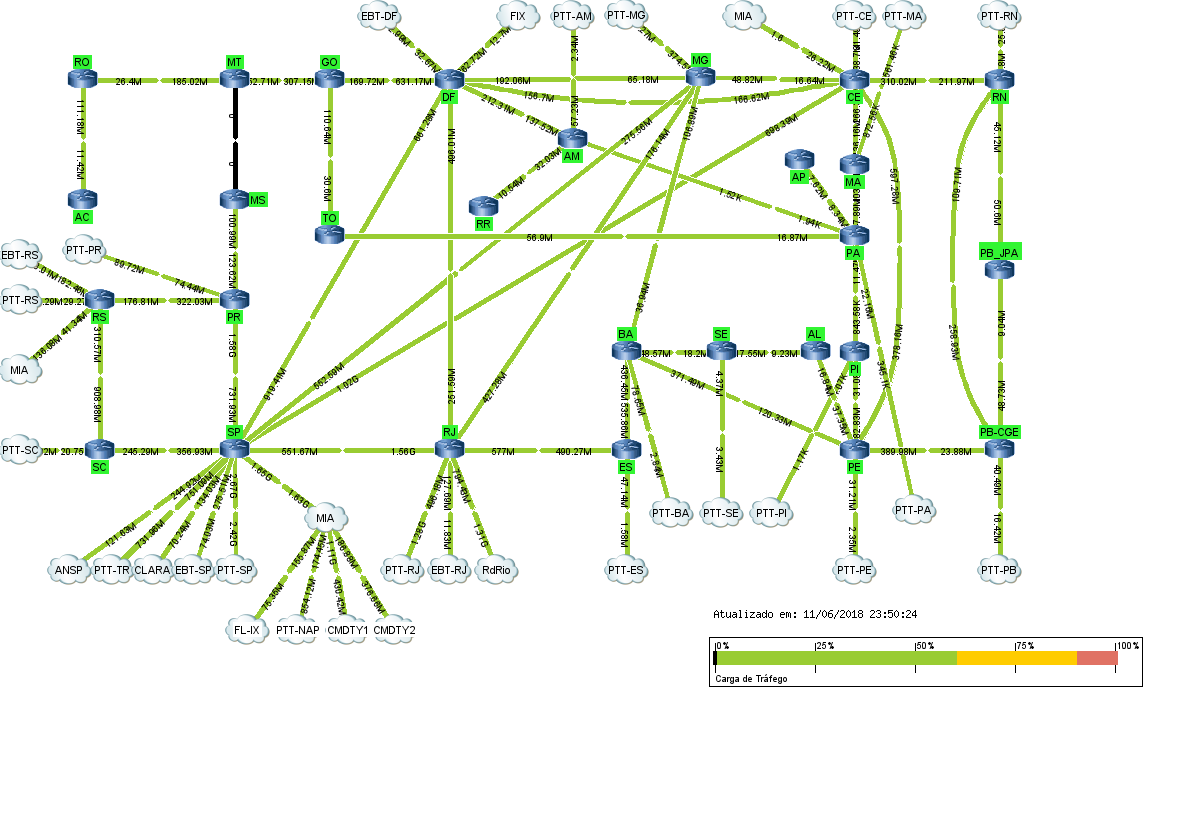
\includegraphics[width=0.8\textwidth]{Imagens/rnp}
  \caption{\label{fig:rnp} Roteadores interno do sistema aut\^onomo da RNP}
\end{figure}

Como n\~ao temos uma rede de malha completa, \'e necess\'ario a utiliza\c{c}\~ao do conceito de refletor de rotas (\textit{route reflector}), onde os roteadores \textit{SP}, \textit{DF}, \textit{MG} e \textit{CE} s\~ao refletores de rotas dos seus roteadores vizinhos, e esses vizinhos sendo refletores de rotas dos pr\'oximos, assim em diante, at\'e abranger todos os roteadores. No nosso projeto, temos que os roteadores \textit{SP}, \textit{DF}, \textit{RS}, \textit{CE}, fazem peering com o AS da Embratel e os roteadores \textit{SP}, \textit{RS}, \textit{CE}, fazem peering com o AS da I2. Esses roteadores que fazem peering com os outros sistemas aut\^onomos exportam rotas pertencentes a cada roteador da rede RNP, e como temos v\'arias sa\'idas para cada um dos ASes, para que seja escolhida o caminho, torna-se necess\'ario a utiliza\c{c}\~ao do atributo MED, tal que o valor MED exportado de cada rota, \'e o valor do custo do roteador que exporta o prefixo para o AS vizinho, at\'e o roteador de origem do mesmo.

\begin{figure}[!htb]
 \centering
 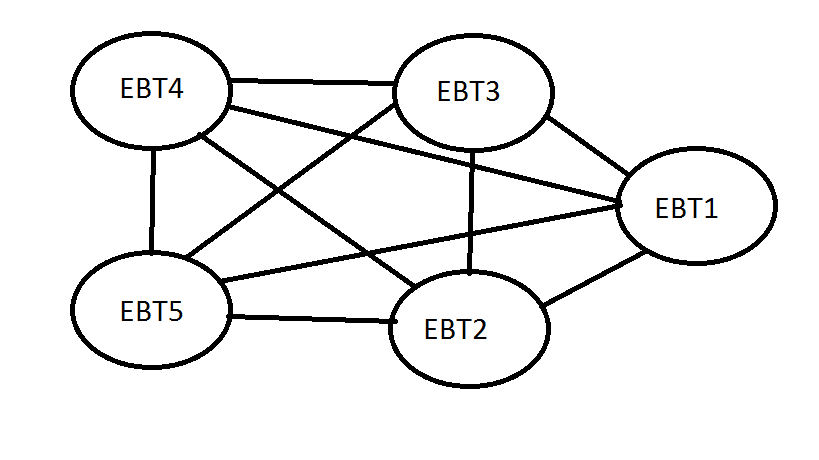
\includegraphics[width=0.5\textwidth]{Imagens/EMBRATEL}
  \caption{\label{fig:Embratel} Roteadores internos simulados que fazem parte do sistema aut\^onomo da Embratel}
\end{figure}

J\'a o sistema aut\^onomo da Embratel consiste em uma rede de malha completa, contendo cinco roteadores, em que o roteador \textit{EBT1} faz peering com um roteador da rede I2 e com o roteador \textit{SP} da RNP , o roteador \textit{EBT2} faz peering com o roteador \textit{CE} da RNP, o roteador \textit{EBT3} faz peering com o roteador do AS BF (Backbone Final), o roteador EBT4 faz peering com o roteador \textit{RS} da RNP, e por fim o roteador \textit{EBT5} faz peering com o roteador \textit{DF} da RNP. A respeito do peering entre o AS da Embratel com o AS da RNP, temos uma rela\c{c}\~ao pol\'itica de exporta\c{c}\~ao, no qual as rotas exportadas do AS da Embratel para a RNP, n\~ao podem ser exportadas para nenhum outro AS.

\begin{figure}[!htb]
 \centering
 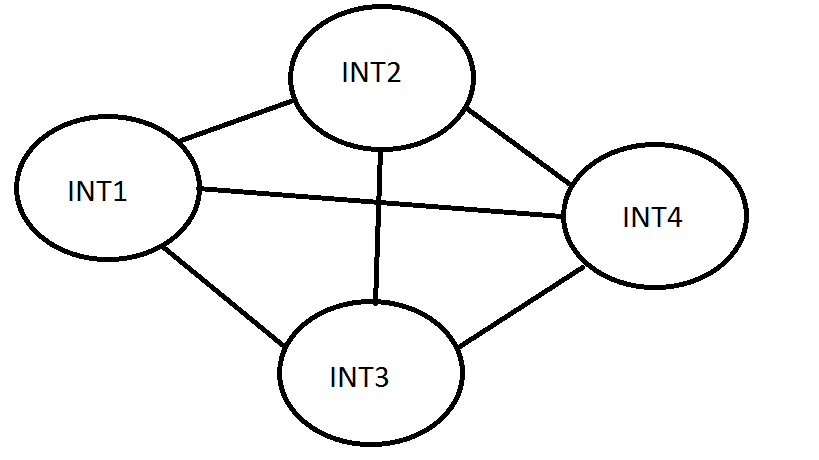
\includegraphics[width=0.5\textwidth]{Imagens/I2_1_}
  \caption{\label{fig:Internet Comercial 2} Roteadores internos simulados que fazem parte do sistema aut\^onomo I2}
\end{figure}

O sistema aut\^onomo I2 (Internet Comercial 2), representa uma rede de malha completa, contendo quatro roteadores. O roteador \textit{INT1} faz peering com o AS da Embratel e com o roteador \textit{SP} da RNP, o roteador \textit{INT2} faz peering com o roteador do AS BF(backbone final), j\'a o roteador \textit{INT3} faz peering com o roteador \textit{CE} da RNP, e por fim o roteador \textit{INT4}, que faz peering com \textit{RS} da RNP. A respeito do peering entre o AS da I2 com o AS da RNP, temos uma rela\c{c}\~ao pol\'itica de exporta\c{c}\~ao de rotas, em que as rotas exportadas do AS da I2 para a RNP, n\~ao podem ser exportadas para nenhum outro AS.

E por fim o AS BF (Backbone final), representado apenas por um roteador que faz peering com os ASes da Embratel e I2, o objetivo desse sistema aut\^onomo \'e visualizar a tomada de decis\~ao do melhor caminho para as rotas originadas do AS da RNP, visto que temos dois caminhos, atrav\'es do AS da Embratel ou do AS da I2. A decis\~ao da melhor rota \'e feita a partir do primeiro crit\'erio, que se refere ao maior valor do LocalPref tem a prefer\^encia mais relevante.

A implementa\c{c}\~ao desses quatro sistemas aut\^onomos foi feita a partir de duas partes, o plano de dados e o plano de controle. O kernel do Linux foi encarregado na parte do plano de dados, ou seja, a cria\c{c}\~ao dos roteadores, interfaces, links de enlace e atribui\c{c}\~oes de endere\c{c}os criados utilizando o Linux Network Namespace. O software BIRD foi respons\'avel pelo plano de controle, ou seja, o BIRD \'e respons\'avel pela defini\c{c}\~ao dos protocolos de roteamento que foram usados, manuseando cada protocolo para que cada roteador realize o seu trabalho de forma correta, e o relacionamento entre os roteadores criados.

O nome "BIRD" \'e na verdade um acr\^onimo para "BIRD Internet Routing Daemon". Pela defini\c{c}\~ao encontrada no site dos desenvolvedores, o BIRD \'e um programa que funciona como um roteador din\^amico em uma rede do tipo Internet (isto \'e, em uma rede que executa o protocolo IPv4 ou IPv6). Os roteadores s\~ao dispositivos que encaminham pacotes entre redes interconectadas para permitir que hosts n\~ao conectados diretamente \`a mesma rede local se comuniquem uns com os outros. Eles tamb\'em se comunicam com os outros roteadores na Internet para descobrir a topologia da rede que permite encontrar regras \'otimas (em termos de algumas m\'etricas) para o encaminhamento de pacotes (que s\~ao chamados de tabelas de roteamento) e se adaptar \`as condi\c{c}\~oes de mudan\c{c}a, como interrup\c{c}\~oes de links de rede, constru\c{c}\~ao de novas conex\~oes e assim por diante. A maioria desses roteadores s\~ao dispositivos dedicados e dispendiosos que executam firmware obscuro, dif\'icil de configurar e que n\~ao se abrem a nenhuma altera\c{c}\~ao.\cite{BIRD} 

Introduzido em 2002, na vers\~ao 2.4.19 do kernel Linux, Namespace \'e um recurso que permite criar e lidar com diversos contextos em um mesmo sistema, vendo propriedades globais diferentes e isoladas em cada contexto, ou seja, permite criar diferentes ambientes independentes que s\~ao executados no sistema base. Para a cria\c{c}\~ao desses ambientes s\~ao utilizados alguns recursos do Namespace\cite{namespace}, tal como: mount namespaces (\textit{mnt}), process id namespaces (\textit{pid}), unix timesharing system namespace (\textit{uts}), network namespace (\textit{net}), inter-process comunication namespace (\textit{ipc}), user namespace (\textit{usr}). O mount namespaces \'e respons\'avel por criar um ambiente isolado para os dispositivos que podem ser montados pelo sistema\cite{mount}. O pid \'e um indetificador de cada processo do kernel\cite{pid}. O uts namespace \'e um recurso usado para isolar dois elementos espec\'ificos do sistemas que se relacionam com uma chamada de sistema\cite{namespace}. Network namespaces permite criar um ambiente de rede isolado do ambiente f\'isico, nesse ambiente existir\~ao interfaces de rede f\'isica, que possuem endere\c{c}os f\'isicos e l\'ogicos diferentes\cite{net}. O ipc namespace tem o intuito de isolar processos de comunica\c{c}\~ao\cite{namespace}. O user namespace \'e respons\'avel pelo isolamento dos identificadores e atributos relacionados \`a seguran\c{c}a.\cite{user}

\chapter{Avalia\c{c}\~ao da Implementa\c{c}\~ao}

Para apresentar a avalia\c{c}\~ao da implementa\c{c}\~ao, vamos mostrar nesta se\c{c}\~ao, as tomadas de decis\~ao realizadas pelos sistemas aut\^onomos implementados, tal como a comunica\c{c}\~ao interna, utiliza\c{c}\~ao do route reflector, a\c{c}\~ao do protocolo iBGP, import\^ancia do atributo MED no protocolo eBGP, implementa\c{c}\~oes de pol\'iticas a partir do atributo community, e a atua\c{c}\~ao do valor do LocalPref. Para demonstrar o comportamento desses aspectos, foi utilizado os recursos \textit{traceroute} (Rastreia a rota de um pacote atrav\'es de uma rede de computadores que utiliza os protocolos IP e o ICMP), \textit{fping} (Encontra as m\'aquinas conectadas e ligadas em uma rede) e as tabelas de roteamento dos roteadores criados.  

Como j\'a foi dito nos cap\'itulos anteriores, o protocolo usado para a comunica\c{c}\~ao interna foi o OSPF, em que a fun\c{c}\~ao dele \'e calcular os saltos de um roteador para outro, e escolher o de menor caminho. Na implementa\c{c}\~ao, cada salto de um roteador para outro tem um custo de valor 5, e o custo do salto para o endere\c{c}o privado de cada roteador \'e de 1. Como exemplo, o caminho do roteador \textit{AC} at\'e o roteador \textit{RJ}, temos o custo de 26, como visto na Figura 5.1 atrav\'es do atributo "OSPF.metric", pois temos 5 saltos entre esses roteador e o custo de mais um para acessar o endere\c{c}o privado do roteador \textit{RJ}, pode ser visto na parte superior da Figura \ref{fig:imagem9}.

\begin{figure}[!htb]
 \centering
 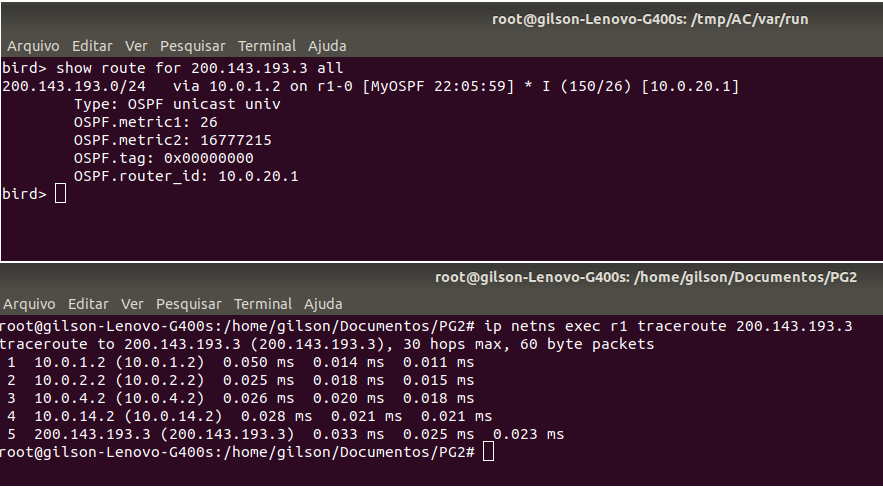
\includegraphics[width=0.5\textwidth]{Imagens/IMAGEM9}
  \caption{\label{fig:imagem9} A parte superior da imagem, mostra as informa\c{c}\~oes da tabela de roteamento do roteador \textit{AC}, para o prefixo que \'e originado pelo roteador \textit{RJ}. A parte inferior da imagem, mostra os saltos, a partir do roteador \textit{AC} at\'e o \textit{RJ}.}
\end{figure}

A Figura \ref{fig:imagem9} \'e divida por duas imagens, no qual a primeira, podemos ver o custo do roteador \textit{AC} at\'e o roteador \textit{RJ}, em que o prefixo \textit{200.143.193.0/24} pertence ao roteador \textit{RJ}. Como visto na imagem, esse custo \'e 26, podemos visualizar isso, a partir do campo \textit{OSPF.metric1}. J\'a a imagem de baixo, representa os saltos que o roteador \textit{AC} deve realizar para se comunicar com o roteador \textit{RJ}. Os endere\c{c}os \textit{10.0.1.2, 10.0.2.2, 10.0.4.2, 10.0.14.2, 200.143.193.0/24}, representam os links de enlace dos roteadores \textit{RO}, \textit{MT}, \textit{GO}, \textit{DF} e \textit{RJ}, respectivamente.

Conforme a se\c{c}\~ao anterior, a utiliza\c{c}\~ao do recurso route reflector foi a partir dos roteadores \textit{SP}, \textit{MG}, \textit{DF}, \textit{CE}, para os seus vizinho e assim em diante, formando assim uma lista de refletores de rotas at\'e o seu destino. Temos um prefixo exportado pelo AS da Embratel, e transmitido entre os roteadores internos pelo protocolo iBGP.

\begin{figure}[!htb]
 \centering
 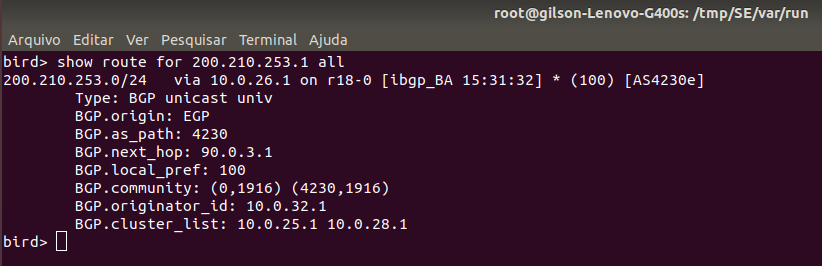
\includegraphics[width=0.7\textwidth]{Imagens/ROUTERREFLECTOR}
  \caption{\label{fig:routerreflector} A imagem de cima, mostra as informa\c{c}\~oes da tabela de roteamento do roteador \textit{SE}, para o prefixo que \'e originado pelo roteador \textit{EBT1} da AS da Embratel.}
\end{figure}

Com a Figura \ref{fig:routerreflector}, atrav\'es do atributo "BGP.cluster", podemos ver a lista de identificadores dos roteadores que funcionam como refletores de rota. At\'e o roteador vizinho do ID pertencente ao atributo "BGP.originator". Os prefixos \textit{10.0.25.1, 10.0.28.1} s\~ao os n\'umeros de ID dos roteadores \textit{BA}, \textit{MG}, respectivamente. Ou seja, o roteador \textit{MG} reflete as rotas para o roteador \textit{BA}, e o roteador \textit{BA} reflete as rotas para o roteador \textit{SE}, assim sendo poss\'ivel uma comunica\c{c}\~ao do protocolo iBGP de forma correta com outros roteadores da rede. O ID de n\'umero \textit{10.0.32.1} pertence ao roteador \textit{CE}, que faz peering com o roteador \textit{EBT2} do AS da Embratel. Logo, para comuni\c{c}\~ao do roteador "SE" para o roteador \textit{EBT1}, passa pelo roteador de borda \textit{CE}.

A utiliza\c{c}\~ao do atributo MED torna-se necess\'ario, pois nos sistemas aut\^onomos da Embratel e da I2, temos m\'ultiplas sa\'idas para a rede da RNP. Como foi visto na se\c{c}\~ao 3, o quarto crit\'erio de escolha na melhor rota \'e o valor MED, tal que o ponto de sa\'ida com o valor do MED mais baixo \'e preferido. Para a atribui\c{c}\~ao desse valor, foi usado o custo calculado pelo protocolo OSPF, como \'e feito na comunica\c{c}\~ao interna, e esse custo de cada rota \'e exportado para outros ASes como o valor do atributo MED.

Para o roteador que importa essas rotas com os atributos MED exportam para os seus vizinhos da mesma rede esses prefixos, no qual o roteador escolhe a rota que possuir o menor valor MED. Como podemos visualizar na Figura \ref{fig:imagem10}.
\\
\\
\\
\\
\\
\\
\\
\\
\\
\begin{figure}[!htb]
 \centering
 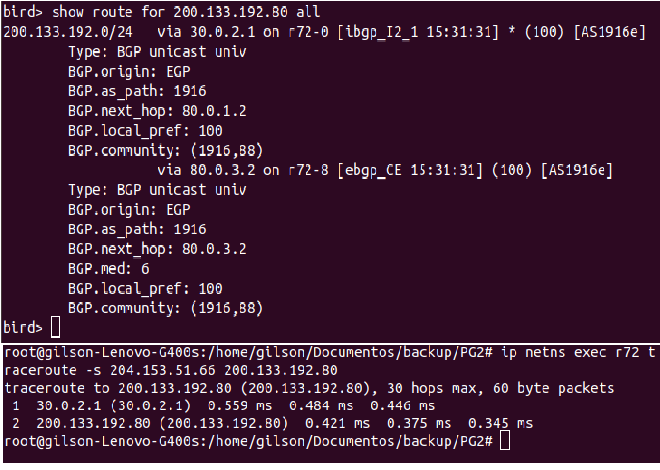
\includegraphics[width=0.5\textwidth]{Imagens/figura63}
  \caption{\label{fig:imagem10} A imagem de cima mostra as informa\c{c}\~oes da tabela de roteamento do roteador \textit{INT3}, para o prefixo que \'e originado pelo roteador \textit{SP} do AS da RNP, e a rota de um pacote a partir do roteador \textit{INT3} at\'e \textit{SP}}
\end{figure}

Na imagem acima, podemos visualizar como o atributo MED fez a diferen\c{c}a, na escolha do melhor caminho do roteador "INT3" para o prefixo \textit{200.133.192.80/24}, pertencente ao roteador \textit{SP} do sistema aut\^onomo da RNP. Temos duas rotas, uma com o valor MED nulo, e a outro com o valor do atributo MED igual a 6. Isso porque a rota com o valor do MED nulo foi exportada pelo roteador \textit{INT1}(\textit{30.0.2.1}) devido o protocolo "ibgp\_I2\_1", onde o \textit{INT1} realiza o peering com o roteador \textit{SP}, logo como faz conex\~ao direta, o custo do valor MED \'e nulo. J\'a o roteador \textit{CE} exporta o valor MED com o mesmo custo at\'e o roteador \textit{SP}. Por fim o roteador \textit{INT3} escolhe com a prioridade mais alta, a rota que possui o valor MED nulo.

Conforme j\'a foi dito na se\c{c}\~ao 3.4, a funcionalidade do atributo community consiste que as rotas exportadas do AS da EBT para o AS da RNP n\~ao podem ser exportadas para num sistema aut\^onomo, o mesmo vale com o AS da I2, onde as rotas exportadas para a RNP, tamb\'em n\~ao podem ser exportadas para outros AS'es. Para cada rota que pertence a essa pol\'itica, \'e marcada com o valor 0 e com o n\'umero do AS a qual vai importar, e a partir de uma tomada de decis\~ao, essa rota \'e exportada ou n\~ao. A Figura \ref{fig:imagem11} mostra a visualiza\c{c}\~ao da marca\c{c}\~ao das rotas.
\\
\\
\\
\\
\\
\\
\\
\\
\\
\\
\\
\\
\\
\\
\\
\\
\\
\begin{figure}[!htb]
 \centering
 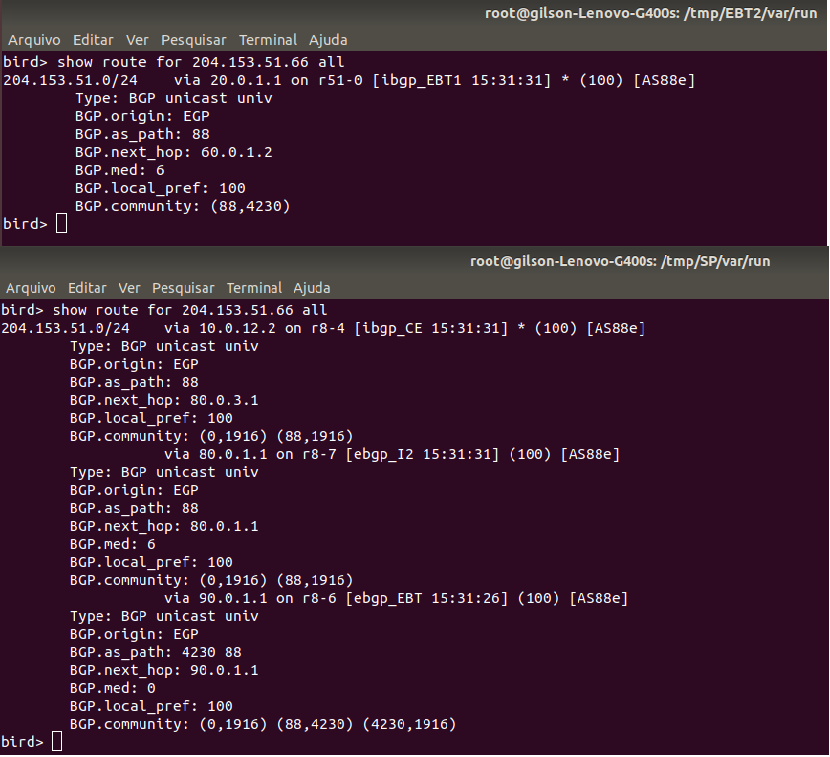
\includegraphics[width=0.5\textwidth]{Imagens/COMMUNITY}
  \caption{\label{fig:imagem11} A imagem de cima, mostram duas imagens, a de cima monstra mostra as informa\c{c}\~oes da tabela de roteamento do roteador \textit{EBT2}, para o prefixo \textit{204.153.51.66} pertencente ao roteador \textit{INT3}. a imagem de baixo mostra as informa\c{c}\~oes da tabela de roteamento do roteador \textit{SP}, para o mesmo prefixo da imagem de cima.}
\end{figure}

Com a Figura \ref{fig:imagem11} podemos visualizar na parte inferior da imagem, que as rotas do AS I2, s\~ao marcadas com dois atributos community, em que um \'e marcado com \textit{(0, 1916)}, significa que o AS de n\'umero 1916 (RNP) n\~ao pode exportar essa rota nenhum outro sistema aut\^onomo, e o segundo atributo marcado \textit{(88,1916)}, significa que essa rota pode ser importada do AS 88 (I2) para o AS 1916 (RNP). J\'a na imagem de cima mostra que essa rota que foi marcada com esse atributo community n\~ao foi exportada do AS da RNP para o AS da EBT.

E por fim, apresentaremos o primeiro crit\'erio de escolha do melhor caminho. Para isso selecionamos todas as rotas que o BF importa do AS da Embratel, com um valor de LocalPref maior que as rotas importadas do AS da I2. Na Figura \ref{fig:imagem12}, podemos ver o valor do LocalPref decidindo a escolha do caminho para tal prefixo.
\\
\\
\\
\\
\\
\\
\\
\\
\\
\\
\\
\\
\begin{figure}[!htb]
 \centering
 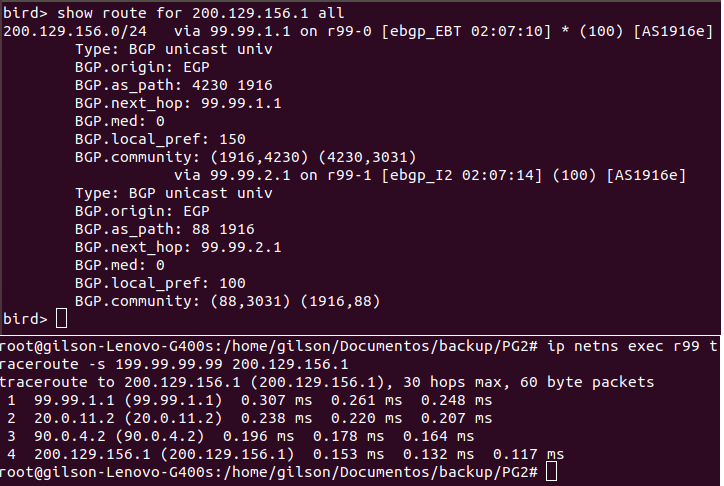
\includegraphics[width=0.5\textwidth]{Imagens/figura65}
  \caption{\label{fig:imagem12} A imagem mostra a tabela de roteamento e a rota de m pacote sa\'ido do roteador da rede BF (representado com o nome \textit{FN}), para o prefixo \textit{200.129.156.1}, pertencente ao roteador \textit{AM} do AS da RNP.}

\end{figure}

A partir da Figura \ref{fig:imagem12}, podemos verificar como o atributo LocalPref influencia na decis\~ao do caminho para um prefixo, onde temos o valor desse atributo vindo do AS da Embratel igual a 150, j\'a o valor de prefer\^encia local vindo do AS da I2 \'e igual a 100. Portanto para o roteador do BF se comunicar com qualquer roteador da RNP, essa comunica\c{c}\~ao passar\'a preferencialmente pela rede da Embratel, devido ao valor de prefer\^encia local ser maior, sendo mostrado na parte inferior da figura, no qual os saltos de um pacote, a partir do BF at\'e AM segue a ordem dos roteadores \textit{99.99.1.1}(BF), \textit{20.0.11.2}(EBT5), \textit{90.0.4.2}(DF), \textit{200.129.156.1}(AM).

\chapter{Conclus\~ao}
Este projeto abordou aspectos relevantes do protocolo BGP e a sua utilidade entre os roteadores de borda, com o intuito de interligar as redes de sistemas aut\^onomos diferentes. Com o objetivo de estudar o entendimento de como \'e o funcionamento dessa comunica\c{c}\~ao, apresentou-se nesse trabalho, aspectos espec\'ificos do funcionamento do protocolo, exibindo m\'etodos de exporta\c{c}\~ao e importa\c{c}\~ao de prefixos, configura\c{c}\~ao das tabelas de roteamento.

Da mesma forma, esse projeto apresentou brevemente, os passos b\'asicos das configura\c{c}\~oes necess\'arias para obter o objetivo geral deste trabalho, que possibilita a cria\c{c}\~ao e a configura\c{c}\~ao de uma topologia utilizando o protocolo BGP nos roteadores que fazem essa comunica\c{c}\~ao com outros ASes. Onde pode ser aplicado em um ambiente real, podendo interligar cidades, pa\'ises, continentes, regi\~oes e etc. Melhorando a qualidade de conex\~ao e transfer\^encia de dados entre essas redes.

Com os conhecimentos apresentados, o objetivo desse projeto foi alcan\c{c}ado, pois \'e poss\'ivel demonstrar as necessidades da implementa\c{c}\~ao e investimentos necess\'arios para a uma configura\c{c}\~ao baseada em neg\'ocios, bom como as aplica\c{c}\~oes de pol\'iticas necess\'arios para a configura\c{c}\~ao e manuten\c{c}\~ao de um ambiente de roteadores, possibilitando uma melhor sa\'ida de dados para as aplica\c{c}\~oes da internet.

\bibliographystyle{abbrv}
\bibliography{bibliografia}

\nocite{*}
\end{document}
